% Dupplicated from https://code.visualstudio.com/docs/remote/containers
\documentclass[11pt]{standalone}
\usepackage[T1]{fontenc}
\usepackage{tikz}
\usetikzlibrary{calc,positioning,shapes.geometric}
\begin{document}
  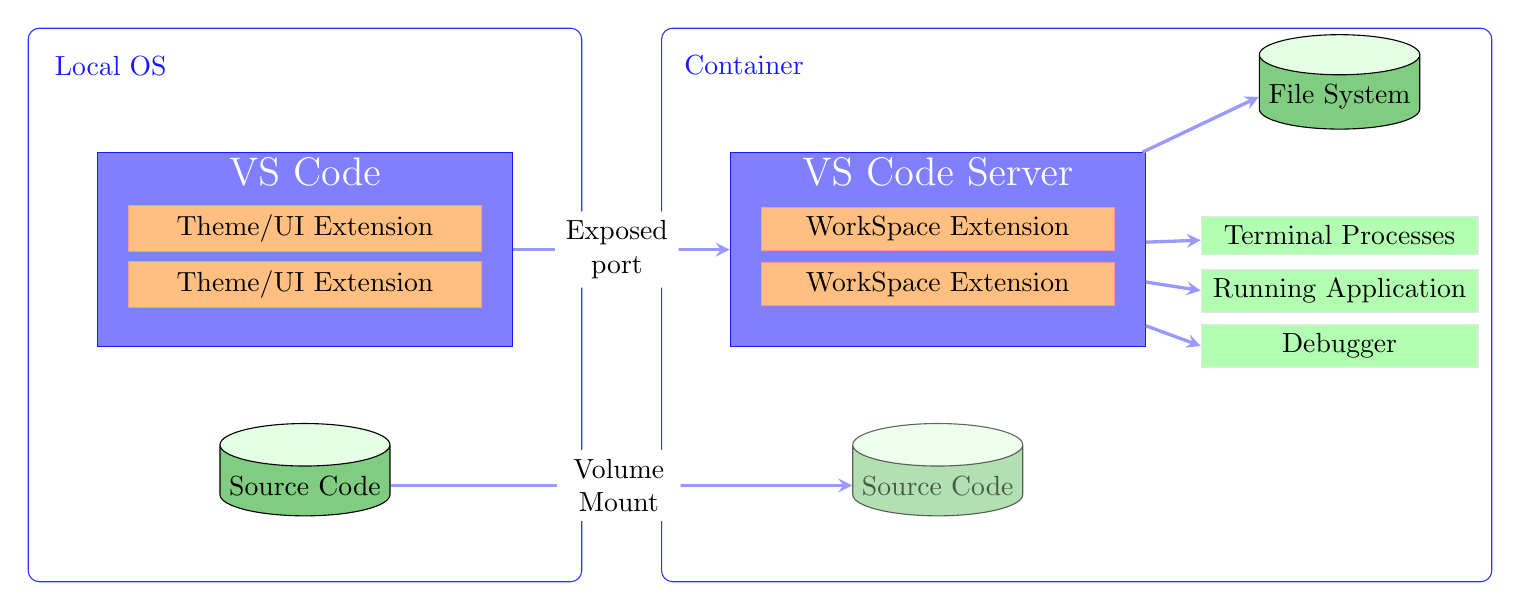
\begin{tikzpicture}[
    >=stealth,
    node distance=1cm,
    orange/.style={
      minimum width = 11em,
      fill=orange!50,
      draw=red!40,
      text width = 0.35\textwidth,
      text centered,
    },
    database/.style={
      cylinder,
      cylinder uses custom fill,
      cylinder body fill=green!60!black!50,
      cylinder end fill=green!10,
      shape border rotate=90,
      aspect=0.25,
      draw
    }
  ]
   
    \node[rounded corners, %fill=black,
    text depth = 5em,
    draw=blue!80,
    % double distance =1pt,    %% here
    %font=\Large, 
    minimum height= 20em,
    minimum width= 20em,
    label={[anchor=north, color=blue!90, inner sep=0pt, xshift=3em, yshift=-1em] north west:{Local OS}}]  (dw){};
    
        \node[rounded corners, %fill=black,
    text depth = 5em,
    draw=blue!80,
    % double distance =1pt,    %% here
    %font=\Large, 
    minimum height= 20em,
    minimum width= 30em,
    label={[anchor=north, color=blue!90, inner sep=0pt, xshift=3em, yshift=-1em] north west:{Container}},
    right = of dw]  (container){};
    \node[ %fill=black,
    draw=blue!90,
    text centered,
    text width = 0.20\textwidth,
    fill=blue!50,
    minimum height= 7em,
    minimum width= 15em,
    label={[anchor=north, inner sep=0pt, yshift=-0.2em] north:{\Large \textcolor{white}{VS Code}}}] at ([yshift=2em] dw.center) (code){};
    \node[orange] at ([yshift=-1.25em] code.center) (t1) {Theme/UI Extension} ;
    \node[orange] at ([yshift= 0.75em] code.center) (t2) {Theme/UI Extension};
  
    \node[ %fill=black,
    draw=blue!90,
    text centered,
    text width = 0.20\textwidth,
    fill=blue!50,
    minimum height= 7em,
    minimum width= 15em,
    label={[anchor=north, inner sep=0pt, yshift=-0.2em] north:{\Large \textcolor{white}{VS Code Server}}}] at ([xshift=10em, yshift=2em] container.west) (codeserver){};
    \node[orange] at ([yshift=-1.25em] codeserver.center) (we1) {WorkSpace Extension} ;
    \node[orange] at ([yshift= 0.75em] codeserver.center) (we2) {WorkSpace Extension};
    
    % Data Sources
      
    % Source Code
    \node[database] (db1) at ([yshift=-5em] code.south) (scOS) {Source Code};
    \node[database, opacity=0.6] (db1) at ([yshift=-5em] codeserver.south) (scContainer) {Source Code};
    % Container Stuff

    % Container widgets
        % Configuration Files and Plugin box
    \node[
    draw=black!10,
    text centered,
    fill=green!30,
    minimum width= 10em] at ([xshift=7em, yshift=-3em] codeserver.north east) (tp){Terminal Processes};
        \node[
    draw=black!10,
    text centered,
    fill=green!30,
    minimum width= 10em] at ([xshift=7em, yshift=-5em] codeserver.north east) (ra){Running Application};
            \node[
    draw=black!10,
    text centered,
    fill=green!30,
    minimum width= 10em] at ([xshift=7em, yshift=-7em] codeserver.north east) (debug){Debugger};
    
     \node[database] (db1) at ([yshift=2em, xshift=7em] codeserver.north east) (fs) {File System};
     
     % Connect and labels
    
    % Arrows 
    \draw[->, very thick, draw=blue!40] (code.east) -> (codeserver.west);
    % Labels
    \node[rounded corners, %fill=black,
    draw=none,
    minimum height= 2em,
    fill = white,
    % double distance =1pt,    %% here
    %font=\Large, 
    text width = 0.11\textwidth,
    text centered,
    minimum width=1.5em,
    xshift=3.75em] at (code.east) (dw1){Exposed port};
    
    \draw[->, very thick, draw=blue!40] (scOS.east) -> (scContainer.west);
    \node[rounded corners, %fill=black,
    draw=none,
    minimum height= 2em,
    fill = white,
    % double distance =1pt,    %% here
    %font=\Large, 
    text width = 0.11\textwidth,
    text centered,
    minimum width=1.5em,
    xshift=8.25em] at (scOS.east) (dw1){Volume Mount};
    \draw[->, very thick, draw=blue!40] (codeserver) -> (fs.west);
    \draw[->, very thick, draw=blue!40] (codeserver) -> (tp);
    \draw[->, very thick, draw=blue!40] (codeserver) -> (ra.west);
    \draw[->, very thick, draw=blue!40] (codeserver) -> (debug.west);
    \end{tikzpicture}
\end{document}